\documentclass[1p]{elsarticle_modified}
%\bibliographystyle{elsarticle-num}

%\usepackage[colorlinks]{hyperref}
%\usepackage{abbrmath_seonhwa} %\Abb, \Ascr, \Acal ,\Abf, \Afrak
\usepackage{amsfonts}
\usepackage{amssymb}
\usepackage{amsmath}
\usepackage{amsthm}
\usepackage{scalefnt}
\usepackage{amsbsy}
\usepackage{kotex}
\usepackage{caption}
\usepackage{subfig}
\usepackage{color}
\usepackage{graphicx}
\usepackage{xcolor} %% white, black, red, green, blue, cyan, magenta, yellow
\usepackage{float}
\usepackage{setspace}
\usepackage{hyperref}

\usepackage{tikz}
\usetikzlibrary{arrows}

\usepackage{multirow}
\usepackage{array} % fixed length table
\usepackage{hhline}

%%%%%%%%%%%%%%%%%%%%%
\makeatletter
\renewcommand*\env@matrix[1][\arraystretch]{%
	\edef\arraystretch{#1}%
	\hskip -\arraycolsep
	\let\@ifnextchar\new@ifnextchar
	\array{*\c@MaxMatrixCols c}}
\makeatother %https://tex.stackexchange.com/questions/14071/how-can-i-increase-the-line-spacing-in-a-matrix
%%%%%%%%%%%%%%%

\usepackage[normalem]{ulem}

\newcommand{\msout}[1]{\ifmmode\text{\sout{\ensuremath{#1}}}\else\sout{#1}\fi}
%SOURCE: \msout is \stkout macro in https://tex.stackexchange.com/questions/20609/strikeout-in-math-mode

\newcommand{\cancel}[1]{
	\ifmmode
	{\color{red}\msout{#1}}
	\else
	{\color{red}\sout{#1}}
	\fi
}

\newcommand{\add}[1]{
	{\color{blue}\uwave{#1}}
}

\newcommand{\replace}[2]{
	\ifmmode
	{\color{red}\msout{#1}}{\color{blue}\uwave{#2}}
	\else
	{\color{red}\sout{#1}}{\color{blue}\uwave{#2}}
	\fi
}

\newcommand{\Sol}{\mathcal{S}} %segment
\newcommand{\D}{D} %diagram
\newcommand{\A}{\mathcal{A}} %arc


%%%%%%%%%%%%%%%%%%%%%%%%%%%%%5 test

\def\sl{\operatorname{\textup{SL}}(2,\Cbb)}
\def\psl{\operatorname{\textup{PSL}}(2,\Cbb)}
\def\quan{\mkern 1mu \triangleright \mkern 1mu}

\theoremstyle{definition}
\newtheorem{thm}{Theorem}[section]
\newtheorem{prop}[thm]{Proposition}
\newtheorem{lem}[thm]{Lemma}
\newtheorem{ques}[thm]{Question}
\newtheorem{cor}[thm]{Corollary}
\newtheorem{defn}[thm]{Definition}
\newtheorem{exam}[thm]{Example}
\newtheorem{rmk}[thm]{Remark}
\newtheorem{alg}[thm]{Algorithm}

\newcommand{\I}{\sqrt{-1}}
\begin{document}

%\begin{frontmatter}
%
%\title{Boundary parabolic representations of knots up to 8 crossings}
%
%%% Group authors per affiliation:
%\author{Yunhi Cho} 
%\address{Department of Mathematics, University of Seoul, Seoul, Korea}
%\ead{yhcho@uos.ac.kr}
%
%
%\author{Seonhwa Kim} %\fnref{s_kim}}
%\address{Center for Geometry and Physics, Institute for Basic Science, Pohang, 37673, Korea}
%\ead{ryeona17@ibs.re.kr}
%
%\author{Hyuk Kim}
%\address{Department of Mathematical Sciences, Seoul National University, Seoul 08826, Korea}
%\ead{hyukkim@snu.ac.kr}
%
%\author{Seokbeom Yoon}
%\address{Department of Mathematical Sciences, Seoul National University, Seoul, 08826,  Korea}
%\ead{sbyoon15@snu.ac.kr}
%
%\begin{abstract}
%We find all boundary parabolic representation of knots up to 8 crossings.
%
%\end{abstract}
%\begin{keyword}
%    \MSC[2010] 57M25 
%\end{keyword}
%
%\end{frontmatter}

%\linenumbers
%\tableofcontents
%
\newcommand\colored[1]{\textcolor{white}{\rule[-0.35ex]{0.8em}{1.4ex}}\kern-0.8em\color{red} #1}%
%\newcommand\colored[1]{\textcolor{white}{ #1}\kern-2.17ex	\textcolor{white}{ #1}\kern-1.81ex	\textcolor{white}{ #1}\kern-2.15ex\color{red}#1	}

{\Large $\underline{11a_{147}~(K11a_{147})}$}

\setlength{\tabcolsep}{10pt}
\renewcommand{\arraystretch}{1.6}
\vspace{1cm}\begin{tabular}{m{100pt}>{\centering\arraybackslash}m{274pt}}
\multirow{5}{120pt}{
	\centering
	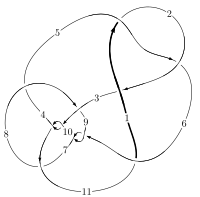
\includegraphics[width=112pt]{../../../GIT/diagram.site/Diagrams/png/396_11a_147.png}\\
\ \ \ A knot diagram\footnotemark}&
\allowdisplaybreaks
\textbf{Linearized knot diagam} \\
\cline{2-2}
 &
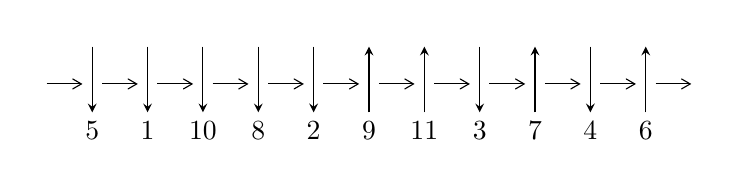
\begin{tikzpicture}[x=20pt, y=17pt]
	% nodes
	\node (C0) at (0, 0) {};
	\node (C1) at (1, 0) {};
	\node (C1U) at (1, +1) {};
	\node (C1D) at (1, -1) {5};

	\node (C2) at (2, 0) {};
	\node (C2U) at (2, +1) {};
	\node (C2D) at (2, -1) {1};

	\node (C3) at (3, 0) {};
	\node (C3U) at (3, +1) {};
	\node (C3D) at (3, -1) {10};

	\node (C4) at (4, 0) {};
	\node (C4U) at (4, +1) {};
	\node (C4D) at (4, -1) {8};

	\node (C5) at (5, 0) {};
	\node (C5U) at (5, +1) {};
	\node (C5D) at (5, -1) {2};

	\node (C6) at (6, 0) {};
	\node (C6U) at (6, +1) {};
	\node (C6D) at (6, -1) {9};

	\node (C7) at (7, 0) {};
	\node (C7U) at (7, +1) {};
	\node (C7D) at (7, -1) {11};

	\node (C8) at (8, 0) {};
	\node (C8U) at (8, +1) {};
	\node (C8D) at (8, -1) {3};

	\node (C9) at (9, 0) {};
	\node (C9U) at (9, +1) {};
	\node (C9D) at (9, -1) {7};

	\node (C10) at (10, 0) {};
	\node (C10U) at (10, +1) {};
	\node (C10D) at (10, -1) {4};

	\node (C11) at (11, 0) {};
	\node (C11U) at (11, +1) {};
	\node (C11D) at (11, -1) {6};
	\node (C12) at (12, 0) {};

	% arrows
	\draw[->,>={angle 60}]
	(C0) edge (C1) (C1) edge (C2) (C2) edge (C3) (C3) edge (C4) (C4) edge (C5) (C5) edge (C6) (C6) edge (C7) (C7) edge (C8) (C8) edge (C9) (C9) edge (C10) (C10) edge (C11) (C11) edge (C12) ;	\draw[->,>=stealth]
	(C1U) edge (C1D) (C2U) edge (C2D) (C3U) edge (C3D) (C4U) edge (C4D) (C5U) edge (C5D) (C6D) edge (C6U) (C7D) edge (C7U) (C8U) edge (C8D) (C9D) edge (C9U) (C10U) edge (C10D) (C11D) edge (C11U) ;
	\end{tikzpicture} \\
\hhline{~~} \\& 
\textbf{Solving Sequence} \\ \cline{2-2} 
 &
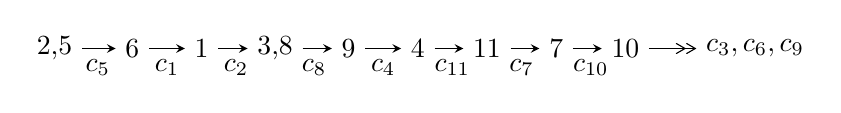
\begin{tikzpicture}[x=25pt, y=7pt]
	% node
	\node (A0) at (-1/8, 0) {2,5};
	\node (A1) at (1, 0) {6};
	\node (A2) at (2, 0) {1};
	\node (A3) at (49/16, 0) {3,8};
	\node (A4) at (33/8, 0) {9};
	\node (A5) at (41/8, 0) {4};
	\node (A6) at (49/8, 0) {11};
	\node (A7) at (57/8, 0) {7};
	\node (A8) at (65/8, 0) {10};
	\node (C1) at (1/2, -1) {$c_{5}$};
	\node (C2) at (3/2, -1) {$c_{1}$};
	\node (C3) at (5/2, -1) {$c_{2}$};
	\node (C4) at (29/8, -1) {$c_{8}$};
	\node (C5) at (37/8, -1) {$c_{4}$};
	\node (C6) at (45/8, -1) {$c_{11}$};
	\node (C7) at (53/8, -1) {$c_{7}$};
	\node (C8) at (61/8, -1) {$c_{10}$};
	\node (A9) at (10, 0) {$c_{3},c_{6},c_{9}$};

	% edge
	\draw[->,>=stealth]	
	(A0) edge (A1) (A1) edge (A2) (A2) edge (A3) (A3) edge (A4) (A4) edge (A5) (A5) edge (A6) (A6) edge (A7) (A7) edge (A8) ;
	\draw[->>,>={angle 60}]	
	(A8) edge (A9);
\end{tikzpicture} \\ 

\end{tabular} \\

\footnotetext{
The image of knot diagram is generated by the software ``\textbf{Draw programme}" developed by Andrew Bartholomew(\url{http://www.layer8.co.uk/maths/draw/index.htm\#Running-draw}), where we modified some parts for our purpose(\url{https://github.com/CATsTAILs/LinksPainter}).
}\phantom \\ \newline 
\centering \textbf{Ideals for irreducible components\footnotemark of $X_{\text{par}}$} 
 
\begin{align*}
I^u_{1}&=\langle 
9.07204\times10^{41} u^{77}+7.90148\times10^{41} u^{76}+\cdots+2.06037\times10^{42} b-1.56482\times10^{41},\\
\phantom{I^u_{1}}&\phantom{= \langle  }1.17116\times10^{42} u^{77}+1.73368\times10^{42} u^{76}+\cdots+2.06037\times10^{42} a-6.11073\times10^{42},\;u^{78}+2 u^{77}+\cdots-2 u-1\rangle \\
I^u_{2}&=\langle 
b,\;-3 u^2+5 a+7 u-6,\;u^3- u^2+1\rangle \\
\\
\end{align*}
\raggedright * 2 irreducible components of $\dim_{\mathbb{C}}=0$, with total 81 representations.\\
\footnotetext{All coefficients of polynomials are rational numbers. But the coefficients are sometimes approximated in decimal forms when there is not enough margin.}
\newpage
\renewcommand{\arraystretch}{1}
\centering \section*{I. $I^u_{1}= \langle 9.07\times10^{41} u^{77}+7.90\times10^{41} u^{76}+\cdots+2.06\times10^{42} b-1.56\times10^{41},\;1.17\times10^{42} u^{77}+1.73\times10^{42} u^{76}+\cdots+2.06\times10^{42} a-6.11\times10^{42},\;u^{78}+2 u^{77}+\cdots-2 u-1 \rangle$}
\flushleft \textbf{(i) Arc colorings}\\
\begin{tabular}{m{7pt} m{180pt} m{7pt} m{180pt} }
\flushright $a_{2}=$&$\begin{pmatrix}0\\u\end{pmatrix}$ \\
\flushright $a_{5}=$&$\begin{pmatrix}1\\0\end{pmatrix}$ \\
\flushright $a_{6}=$&$\begin{pmatrix}1\\u^2\end{pmatrix}$ \\
\flushright $a_{1}=$&$\begin{pmatrix}u\\u\end{pmatrix}$ \\
\flushright $a_{3}=$&$\begin{pmatrix}- u^3\\- u^3+u\end{pmatrix}$ \\
\flushright $a_{8}=$&$\begin{pmatrix}-0.568420 u^{77}-0.841443 u^{76}+\cdots+7.36773 u+2.96584\\-0.440311 u^{77}-0.383498 u^{76}+\cdots+0.720857 u+0.0759485\end{pmatrix}$ \\
\flushright $a_{9}=$&$\begin{pmatrix}-1.82193 u^{77}-2.29694 u^{76}+\cdots+8.78768 u+3.83863\\-1.36819 u^{77}-2.06052 u^{76}+\cdots+2.39639 u+1.90814\end{pmatrix}$ \\
\flushright $a_{4}=$&$\begin{pmatrix}-1.18444 u^{77}-2.09711 u^{76}+\cdots+1.00657 u+1.49223\\0.344158 u^{77}+1.17317 u^{76}+\cdots-0.834190 u-1.22870\end{pmatrix}$ \\
\flushright $a_{11}=$&$\begin{pmatrix}u^3\\u^5- u^3+u\end{pmatrix}$ \\
\flushright $a_{7}=$&$\begin{pmatrix}-1.12364 u^{77}-1.00031 u^{76}+\cdots+7.99454 u+3.41779\\-1.37767 u^{77}-1.68487 u^{76}+\cdots+2.56542 u+1.34481\end{pmatrix}$ \\
\flushright $a_{10}=$&$\begin{pmatrix}1.18444 u^{77}+2.09711 u^{76}+\cdots-1.00657 u-1.49223\\0.380290 u^{77}+1.21706 u^{76}+\cdots-0.193293 u-1.50047\end{pmatrix}$\\ \flushright $a_{10}=$&$\begin{pmatrix}1.18444 u^{77}+2.09711 u^{76}+\cdots-1.00657 u-1.49223\\0.380290 u^{77}+1.21706 u^{76}+\cdots-0.193293 u-1.50047\end{pmatrix}$\\&\end{tabular}
\flushleft \textbf{(ii) Obstruction class $= -1$}\\~\\
\flushleft \textbf{(iii) Cusp Shapes $= 3.52017 u^{77}+0.863610 u^{76}+\cdots-23.9616 u-10.9917$}\\~\\
\newpage\renewcommand{\arraystretch}{1}
\flushleft \textbf{(iv) u-Polynomials at the component}\newline \\
\begin{tabular}{m{50pt}|m{274pt}}
Crossings & \hspace{64pt}u-Polynomials at each crossing \\
\hline $$\begin{aligned}c_{1},c_{5}\end{aligned}$$&$\begin{aligned}
&u^{78}+2 u^{77}+\cdots-2 u-1
\end{aligned}$\\
\hline $$\begin{aligned}c_{2}\end{aligned}$$&$\begin{aligned}
&u^{78}+38 u^{77}+\cdots+4 u+1
\end{aligned}$\\
\hline $$\begin{aligned}c_{3},c_{10}\end{aligned}$$&$\begin{aligned}
&u^{78}+2 u^{77}+\cdots+4 u+1
\end{aligned}$\\
\hline $$\begin{aligned}c_{4}\end{aligned}$$&$\begin{aligned}
&u^{78}+3 u^{77}+\cdots+1620 u+200
\end{aligned}$\\
\hline $$\begin{aligned}c_{6},c_{9}\end{aligned}$$&$\begin{aligned}
&u^{78}+4 u^{77}+\cdots-349 u-25
\end{aligned}$\\
\hline $$\begin{aligned}c_{7}\end{aligned}$$&$\begin{aligned}
&5(5 u^{78}+22 u^{77}+\cdots-2074 u-329)
\end{aligned}$\\
\hline $$\begin{aligned}c_{8}\end{aligned}$$&$\begin{aligned}
&5(5 u^{78}-57 u^{77}+\cdots-1179 u-1431)
\end{aligned}$\\
\hline $$\begin{aligned}c_{11}\end{aligned}$$&$\begin{aligned}
&u^{78}+6 u^{77}+\cdots-20170 u-4025
\end{aligned}$\\
\hline
\end{tabular}\\~\\
\newpage\renewcommand{\arraystretch}{1}
\flushleft \textbf{(v) Riley Polynomials at the component}\newline \\
\begin{tabular}{m{50pt}|m{274pt}}
Crossings & \hspace{64pt}Riley Polynomials at each crossing \\
\hline $$\begin{aligned}c_{1},c_{5}\end{aligned}$$&$\begin{aligned}
&y^{78}-38 y^{77}+\cdots-4 y+1
\end{aligned}$\\
\hline $$\begin{aligned}c_{2}\end{aligned}$$&$\begin{aligned}
&y^{78}+6 y^{77}+\cdots+8 y+1
\end{aligned}$\\
\hline $$\begin{aligned}c_{3},c_{10}\end{aligned}$$&$\begin{aligned}
&y^{78}-42 y^{77}+\cdots-4 y+1
\end{aligned}$\\
\hline $$\begin{aligned}c_{4}\end{aligned}$$&$\begin{aligned}
&y^{78}-21 y^{77}+\cdots-354000 y+40000
\end{aligned}$\\
\hline $$\begin{aligned}c_{6},c_{9}\end{aligned}$$&$\begin{aligned}
&y^{78}-44 y^{77}+\cdots-59401 y+625
\end{aligned}$\\
\hline $$\begin{aligned}c_{7}\end{aligned}$$&$\begin{aligned}
&25(25 y^{78}+186 y^{77}+\cdots+726960 y+108241)
\end{aligned}$\\
\hline $$\begin{aligned}c_{8}\end{aligned}$$&$\begin{aligned}
&25(25 y^{78}-499 y^{77}+\cdots-2.01676\times10^{7} y+2047761)
\end{aligned}$\\
\hline $$\begin{aligned}c_{11}\end{aligned}$$&$\begin{aligned}
&y^{78}+26 y^{77}+\cdots-39169300 y+16200625
\end{aligned}$\\
\hline
\end{tabular}\\~\\
\newpage\flushleft \textbf{(vi) Complex Volumes and Cusp Shapes}
$$\begin{array}{c|c|c}  
\text{Solutions to }I^u_{1}& \I (\text{vol} + \sqrt{-1}CS) & \text{Cusp shape}\\
 \hline 
\begin{aligned}
u &= -0.746844 + 0.705544 I \\
a &= -0.478258 - 0.846046 I \\
b &= -0.973201 + 0.859230 I\end{aligned}
 & \phantom{-}1.84214 + 9.51725 I & \phantom{-0.000000 } 0 \\ \hline\begin{aligned}
u &= -0.746844 - 0.705544 I \\
a &= -0.478258 + 0.846046 I \\
b &= -0.973201 - 0.859230 I\end{aligned}
 & \phantom{-}1.84214 - 9.51725 I & \phantom{-0.000000 } 0 \\ \hline\begin{aligned}
u &= \phantom{-}0.733786 + 0.768282 I \\
a &= -0.238190 + 0.368034 I \\
b &= -0.480787 - 0.550929 I\end{aligned}
 & \phantom{-}5.29151 - 3.14059 I & \phantom{-0.000000 } 0 \\ \hline\begin{aligned}
u &= \phantom{-}0.733786 - 0.768282 I \\
a &= -0.238190 - 0.368034 I \\
b &= -0.480787 + 0.550929 I\end{aligned}
 & \phantom{-}5.29151 + 3.14059 I & \phantom{-0.000000 } 0 \\ \hline\begin{aligned}
u &= -1.024600 + 0.336794 I \\
a &= \phantom{-}1.54401 - 1.42228 I \\
b &= \phantom{-}0.01866 - 1.42927 I\end{aligned}
 & -2.14618 - 1.33328 I & \phantom{-0.000000 } 0 \\ \hline\begin{aligned}
u &= -1.024600 - 0.336794 I \\
a &= \phantom{-}1.54401 + 1.42228 I \\
b &= \phantom{-}0.01866 + 1.42927 I\end{aligned}
 & -2.14618 + 1.33328 I & \phantom{-0.000000 } 0 \\ \hline\begin{aligned}
u &= -0.850399 + 0.683748 I \\
a &= -0.505972 + 0.523823 I \\
b &= \phantom{-}0.842741 + 0.745286 I\end{aligned}
 & \phantom{-}1.54329 - 4.25093 I & \phantom{-0.000000 } 0 \\ \hline\begin{aligned}
u &= -0.850399 - 0.683748 I \\
a &= -0.505972 - 0.523823 I \\
b &= \phantom{-}0.842741 - 0.745286 I\end{aligned}
 & \phantom{-}1.54329 + 4.25093 I & \phantom{-0.000000 } 0 \\ \hline\begin{aligned}
u &= -0.739719 + 0.511752 I \\
a &= \phantom{-}0.333454 + 0.752332 I \\
b &= \phantom{-}0.877805 - 0.981944 I\end{aligned}
 & -1.96956 + 4.60975 I & -4.54210 - 7.29697 I \\ \hline\begin{aligned}
u &= -0.739719 - 0.511752 I \\
a &= \phantom{-}0.333454 - 0.752332 I \\
b &= \phantom{-}0.877805 + 0.981944 I\end{aligned}
 & -1.96956 - 4.60975 I & -4.54210 + 7.29697 I\\
 \hline 
 \end{array}$$\newpage$$\begin{array}{c|c|c}  
\text{Solutions to }I^u_{1}& \I (\text{vol} + \sqrt{-1}CS) & \text{Cusp shape}\\
 \hline 
\begin{aligned}
u &= \phantom{-}0.309437 + 0.842121 I \\
a &= -0.303870 - 0.378991 I \\
b &= -0.893991 + 0.759593 I\end{aligned}
 & \phantom{-}2.88434 + 6.11355 I & \phantom{-}0.57263 - 4.98451 I \\ \hline\begin{aligned}
u &= \phantom{-}0.309437 - 0.842121 I \\
a &= -0.303870 + 0.378991 I \\
b &= -0.893991 - 0.759593 I\end{aligned}
 & \phantom{-}2.88434 - 6.11355 I & \phantom{-}0.57263 + 4.98451 I \\ \hline\begin{aligned}
u &= \phantom{-}1.030610 + 0.412848 I \\
a &= \phantom{-}1.68779 - 0.30818 I \\
b &= \phantom{-}0.372068 + 0.975530 I\end{aligned}
 & -0.08665 - 1.81934 I & \phantom{-0.000000 } 0 \\ \hline\begin{aligned}
u &= \phantom{-}1.030610 - 0.412848 I \\
a &= \phantom{-}1.68779 + 0.30818 I \\
b &= \phantom{-}0.372068 - 0.975530 I\end{aligned}
 & -0.08665 + 1.81934 I & \phantom{-0.000000 } 0 \\ \hline\begin{aligned}
u &= -0.289191 + 0.831056 I \\
a &= -0.532023 + 0.563698 I \\
b &= -1.25627 - 0.93792 I\end{aligned}
 & -0.68796 - 12.03560 I & -2.39702 + 6.80252 I \\ \hline\begin{aligned}
u &= -0.289191 - 0.831056 I \\
a &= -0.532023 - 0.563698 I \\
b &= -1.25627 + 0.93792 I\end{aligned}
 & -0.68796 + 12.03560 I & -2.39702 - 6.80252 I \\ \hline\begin{aligned}
u &= \phantom{-}1.017100 + 0.476390 I \\
a &= \phantom{-}2.80013 - 1.11064 I \\
b &= \phantom{-}1.24917 + 0.87506 I\end{aligned}
 & \phantom{-}0.76206 - 1.48191 I & \phantom{-0.000000 } 0 \\ \hline\begin{aligned}
u &= \phantom{-}1.017100 - 0.476390 I \\
a &= \phantom{-}2.80013 + 1.11064 I \\
b &= \phantom{-}1.24917 - 0.87506 I\end{aligned}
 & \phantom{-}0.76206 + 1.48191 I & \phantom{-0.000000 } 0 \\ \hline\begin{aligned}
u &= -0.367142 + 0.771630 I \\
a &= \phantom{-}0.295260 + 0.430720 I \\
b &= -0.826296 - 0.097021 I\end{aligned}
 & -2.74670 - 1.03689 I & -6.52285 + 3.02306 I \\ \hline\begin{aligned}
u &= -0.367142 - 0.771630 I \\
a &= \phantom{-}0.295260 - 0.430720 I \\
b &= -0.826296 + 0.097021 I\end{aligned}
 & -2.74670 + 1.03689 I & -6.52285 - 3.02306 I\\
 \hline 
 \end{array}$$\newpage$$\begin{array}{c|c|c}  
\text{Solutions to }I^u_{1}& \I (\text{vol} + \sqrt{-1}CS) & \text{Cusp shape}\\
 \hline 
\begin{aligned}
u &= -0.149695 + 0.830340 I \\
a &= \phantom{-}0.245507 - 0.296928 I \\
b &= \phantom{-}0.865089 - 0.200429 I\end{aligned}
 & -2.45171 + 2.55877 I & -5.85987 - 5.37138 I \\ \hline\begin{aligned}
u &= -0.149695 - 0.830340 I \\
a &= \phantom{-}0.245507 + 0.296928 I \\
b &= \phantom{-}0.865089 + 0.200429 I\end{aligned}
 & -2.45171 - 2.55877 I & -5.85987 + 5.37138 I \\ \hline\begin{aligned}
u &= -1.088040 + 0.413183 I \\
a &= -1.09001 + 0.98084 I \\
b &= -0.001009 - 0.600156 I\end{aligned}
 & -3.19952 + 3.59888 I & \phantom{-0.000000 } 0 \\ \hline\begin{aligned}
u &= -1.088040 - 0.413183 I \\
a &= -1.09001 - 0.98084 I \\
b &= -0.001009 + 0.600156 I\end{aligned}
 & -3.19952 - 3.59888 I & \phantom{-0.000000 } 0 \\ \hline\begin{aligned}
u &= \phantom{-}1.139890 + 0.236298 I \\
a &= \phantom{-}1.41756 + 0.21010 I \\
b &= \phantom{-}1.132930 + 0.048625 I\end{aligned}
 & -7.37477 - 1.65920 I & \phantom{-0.000000 } 0 \\ \hline\begin{aligned}
u &= \phantom{-}1.139890 - 0.236298 I \\
a &= \phantom{-}1.41756 - 0.21010 I \\
b &= \phantom{-}1.132930 - 0.048625 I\end{aligned}
 & -7.37477 + 1.65920 I & \phantom{-0.000000 } 0 \\ \hline\begin{aligned}
u &= -1.051900 + 0.501021 I \\
a &= \phantom{-}1.93452 + 1.70901 I \\
b &= \phantom{-}1.48871 + 0.16626 I\end{aligned}
 & \phantom{-}1.14399 + 4.70367 I & \phantom{-0.000000 } 0 \\ \hline\begin{aligned}
u &= -1.051900 - 0.501021 I \\
a &= \phantom{-}1.93452 - 1.70901 I \\
b &= \phantom{-}1.48871 - 0.16626 I\end{aligned}
 & \phantom{-}1.14399 - 4.70367 I & \phantom{-0.000000 } 0 \\ \hline\begin{aligned}
u &= -1.078790 + 0.507036 I \\
a &= \phantom{-}0.473785 + 1.201770 I \\
b &= \phantom{-}0.961578 + 0.893094 I\end{aligned}
 & \phantom{-}0.70811 + 4.91347 I & \phantom{-0.000000 } 0 \\ \hline\begin{aligned}
u &= -1.078790 - 0.507036 I \\
a &= \phantom{-}0.473785 - 1.201770 I \\
b &= \phantom{-}0.961578 - 0.893094 I\end{aligned}
 & \phantom{-}0.70811 - 4.91347 I & \phantom{-0.000000 } 0\\
 \hline 
 \end{array}$$\newpage$$\begin{array}{c|c|c}  
\text{Solutions to }I^u_{1}& \I (\text{vol} + \sqrt{-1}CS) & \text{Cusp shape}\\
 \hline 
\begin{aligned}
u &= \phantom{-}0.934335 + 0.746651 I \\
a &= -0.193081 - 0.276408 I \\
b &= \phantom{-}0.385335 - 0.321158 I\end{aligned}
 & \phantom{-}4.74268 - 2.53637 I & \phantom{-0.000000 } 0 \\ \hline\begin{aligned}
u &= \phantom{-}0.934335 - 0.746651 I \\
a &= -0.193081 + 0.276408 I \\
b &= \phantom{-}0.385335 + 0.321158 I\end{aligned}
 & \phantom{-}4.74268 + 2.53637 I & \phantom{-0.000000 } 0 \\ \hline\begin{aligned}
u &= \phantom{-}1.155640 + 0.314214 I \\
a &= -1.98719 + 1.54907 I \\
b &= -1.52907 + 0.68369 I\end{aligned}
 & -8.20158 + 2.35498 I & \phantom{-0.000000 } 0 \\ \hline\begin{aligned}
u &= \phantom{-}1.155640 - 0.314214 I \\
a &= -1.98719 - 1.54907 I \\
b &= -1.52907 - 0.68369 I\end{aligned}
 & -8.20158 - 2.35498 I & \phantom{-0.000000 } 0 \\ \hline\begin{aligned}
u &= \phantom{-}1.105230 + 0.476843 I \\
a &= -1.41172 + 3.06153 I \\
b &= \phantom{-}0.065078 - 0.438552 I\end{aligned}
 & -2.73306 - 3.75480 I & \phantom{-0.000000 } 0 \\ \hline\begin{aligned}
u &= \phantom{-}1.105230 - 0.476843 I \\
a &= -1.41172 - 3.06153 I \\
b &= \phantom{-}0.065078 + 0.438552 I\end{aligned}
 & -2.73306 + 3.75480 I & \phantom{-0.000000 } 0 \\ \hline\begin{aligned}
u &= -1.155380 + 0.357963 I \\
a &= -1.26784 - 0.83955 I \\
b &= -0.924109 - 0.405905 I\end{aligned}
 & -4.19189 + 1.50549 I & \phantom{-0.000000 } 0 \\ \hline\begin{aligned}
u &= -1.155380 - 0.357963 I \\
a &= -1.26784 + 0.83955 I \\
b &= -0.924109 + 0.405905 I\end{aligned}
 & -4.19189 - 1.50549 I & \phantom{-0.000000 } 0 \\ \hline\begin{aligned}
u &= -0.625614 + 0.475003 I \\
a &= \phantom{-}1.41445 - 0.35012 I \\
b &= -0.483183 - 0.492391 I\end{aligned}
 & -1.77605 - 0.65095 I & -5.05775 - 1.02917 I \\ \hline\begin{aligned}
u &= -0.625614 - 0.475003 I \\
a &= \phantom{-}1.41445 + 0.35012 I \\
b &= -0.483183 + 0.492391 I\end{aligned}
 & -1.77605 + 0.65095 I & -5.05775 + 1.02917 I\\
 \hline 
 \end{array}$$\newpage$$\begin{array}{c|c|c}  
\text{Solutions to }I^u_{1}& \I (\text{vol} + \sqrt{-1}CS) & \text{Cusp shape}\\
 \hline 
\begin{aligned}
u &= \phantom{-}1.096640 + 0.524719 I \\
a &= -1.33967 - 1.54913 I \\
b &= \phantom{-}0.48017 - 1.76300 I\end{aligned}
 & -0.80322 - 8.33176 I & \phantom{-0.000000 } 0 \\ \hline\begin{aligned}
u &= \phantom{-}1.096640 - 0.524719 I \\
a &= -1.33967 + 1.54913 I \\
b &= \phantom{-}0.48017 + 1.76300 I\end{aligned}
 & -0.80322 + 8.33176 I & \phantom{-0.000000 } 0 \\ \hline\begin{aligned}
u &= -0.238423 + 0.742435 I \\
a &= \phantom{-}0.513424 - 0.435915 I \\
b &= \phantom{-}1.44532 + 0.92730 I\end{aligned}
 & -4.07487 - 5.63539 I & -5.32059 + 5.07237 I \\ \hline\begin{aligned}
u &= -0.238423 - 0.742435 I \\
a &= \phantom{-}0.513424 + 0.435915 I \\
b &= \phantom{-}1.44532 - 0.92730 I\end{aligned}
 & -4.07487 + 5.63539 I & -5.32059 - 5.07237 I \\ \hline\begin{aligned}
u &= -1.207250 + 0.220796 I \\
a &= \phantom{-}1.27897 + 0.72201 I \\
b &= \phantom{-}0.968015 + 0.543909 I\end{aligned}
 & -2.09592 - 2.91398 I & \phantom{-0.000000 } 0 \\ \hline\begin{aligned}
u &= -1.207250 - 0.220796 I \\
a &= \phantom{-}1.27897 - 0.72201 I \\
b &= \phantom{-}0.968015 - 0.543909 I\end{aligned}
 & -2.09592 + 2.91398 I & \phantom{-0.000000 } 0 \\ \hline\begin{aligned}
u &= \phantom{-}0.653825 + 0.410103 I \\
a &= \phantom{-}0.603104 - 0.900709 I \\
b &= \phantom{-}0.137771 + 0.795666 I\end{aligned}
 & \phantom{-}1.09693 - 1.53880 I & \phantom{-}1.66479 + 5.08310 I \\ \hline\begin{aligned}
u &= \phantom{-}0.653825 - 0.410103 I \\
a &= \phantom{-}0.603104 + 0.900709 I \\
b &= \phantom{-}0.137771 - 0.795666 I\end{aligned}
 & \phantom{-}1.09693 + 1.53880 I & \phantom{-}1.66479 - 5.08310 I \\ \hline\begin{aligned}
u &= \phantom{-}1.207280 + 0.247867 I \\
a &= \phantom{-}1.80061 - 1.10036 I \\
b &= \phantom{-}1.29376 - 0.79776 I\end{aligned}
 & -5.50516 + 8.73601 I & \phantom{-0.000000 } 0 \\ \hline\begin{aligned}
u &= \phantom{-}1.207280 - 0.247867 I \\
a &= \phantom{-}1.80061 + 1.10036 I \\
b &= \phantom{-}1.29376 + 0.79776 I\end{aligned}
 & -5.50516 - 8.73601 I & \phantom{-0.000000 } 0\\
 \hline 
 \end{array}$$\newpage$$\begin{array}{c|c|c}  
\text{Solutions to }I^u_{1}& \I (\text{vol} + \sqrt{-1}CS) & \text{Cusp shape}\\
 \hline 
\begin{aligned}
u &= \phantom{-}1.141590 + 0.513261 I \\
a &= -1.97225 + 0.58221 I \\
b &= -0.883958 - 0.783696 I\end{aligned}
 & -3.10971 - 6.53083 I & \phantom{-0.000000 } 0 \\ \hline\begin{aligned}
u &= \phantom{-}1.141590 - 0.513261 I \\
a &= -1.97225 - 0.58221 I \\
b &= -0.883958 + 0.783696 I\end{aligned}
 & -3.10971 + 6.53083 I & \phantom{-0.000000 } 0 \\ \hline\begin{aligned}
u &= \phantom{-}0.536973 + 0.520683 I \\
a &= -0.275984 - 0.550833 I \\
b &= -0.91164 + 1.14392 I\end{aligned}
 & \phantom{-}2.17308 - 2.60159 I & \phantom{-}2.40455 + 6.09883 I \\ \hline\begin{aligned}
u &= \phantom{-}0.536973 - 0.520683 I \\
a &= -0.275984 + 0.550833 I \\
b &= -0.91164 - 1.14392 I\end{aligned}
 & \phantom{-}2.17308 + 2.60159 I & \phantom{-}2.40455 - 6.09883 I \\ \hline\begin{aligned}
u &= -0.739477\phantom{ +0.000000I} \\
a &= \phantom{-}0.804258\phantom{ +0.000000I} \\
b &= \phantom{-}0.322518\phantom{ +0.000000I}\end{aligned}
 & -0.989802\phantom{ +0.000000I} & -10.9810\phantom{ +0.000000I} \\ \hline\begin{aligned}
u &= \phantom{-}1.214520 + 0.340708 I \\
a &= -1.65330 - 0.02146 I \\
b &= -1.065870 - 0.267377 I\end{aligned}
 & -6.71121 - 6.46472 I & \phantom{-0.000000 } 0 \\ \hline\begin{aligned}
u &= \phantom{-}1.214520 - 0.340708 I \\
a &= -1.65330 + 0.02146 I \\
b &= -1.065870 + 0.267377 I\end{aligned}
 & -6.71121 + 6.46472 I & \phantom{-0.000000 } 0 \\ \hline\begin{aligned}
u &= -1.145480 + 0.533343 I \\
a &= -2.71029 - 1.10644 I \\
b &= -1.59668 + 0.98544 I\end{aligned}
 & -6.70525 + 10.43610 I & \phantom{-0.000000 } 0 \\ \hline\begin{aligned}
u &= -1.145480 - 0.533343 I \\
a &= -2.71029 + 1.10644 I \\
b &= -1.59668 - 0.98544 I\end{aligned}
 & -6.70525 - 10.43610 I & \phantom{-0.000000 } 0 \\ \hline\begin{aligned}
u &= -1.129540 + 0.584934 I \\
a &= \phantom{-}0.773398 + 1.151490 I \\
b &= \phantom{-}0.901036 - 0.260596 I\end{aligned}
 & -5.00368 + 6.17548 I & \phantom{-0.000000 } 0\\
 \hline 
 \end{array}$$\newpage$$\begin{array}{c|c|c}  
\text{Solutions to }I^u_{1}& \I (\text{vol} + \sqrt{-1}CS) & \text{Cusp shape}\\
 \hline 
\begin{aligned}
u &= -1.129540 - 0.584934 I \\
a &= \phantom{-}0.773398 - 1.151490 I \\
b &= \phantom{-}0.901036 + 0.260596 I\end{aligned}
 & -5.00368 - 6.17548 I & \phantom{-0.000000 } 0 \\ \hline\begin{aligned}
u &= \phantom{-}0.193316 + 0.691312 I \\
a &= \phantom{-}0.545322 + 0.428076 I \\
b &= \phantom{-}0.704072 - 0.657723 I\end{aligned}
 & -0.42144 + 1.94552 I & -2.30995 - 3.00822 I \\ \hline\begin{aligned}
u &= \phantom{-}0.193316 - 0.691312 I \\
a &= \phantom{-}0.545322 - 0.428076 I \\
b &= \phantom{-}0.704072 + 0.657723 I\end{aligned}
 & -0.42144 - 1.94552 I & -2.30995 + 3.00822 I \\ \hline\begin{aligned}
u &= \phantom{-}0.325468 + 0.636702 I \\
a &= -0.138810 + 0.488594 I \\
b &= -0.55951 - 1.52885 I\end{aligned}
 & \phantom{-}1.40525 + 3.78104 I & \phantom{-}0.49759 - 6.55380 I \\ \hline\begin{aligned}
u &= \phantom{-}0.325468 - 0.636702 I \\
a &= -0.138810 - 0.488594 I \\
b &= -0.55951 + 1.52885 I\end{aligned}
 & \phantom{-}1.40525 - 3.78104 I & \phantom{-}0.49759 + 6.55380 I \\ \hline\begin{aligned}
u &= -1.187200 + 0.508151 I \\
a &= -1.06426 - 1.06765 I \\
b &= -0.898331 - 0.033808 I\end{aligned}
 & -5.56201 + 2.30321 I & \phantom{-0.000000 } 0 \\ \hline\begin{aligned}
u &= -1.187200 - 0.508151 I \\
a &= -1.06426 + 1.06765 I \\
b &= -0.898331 + 0.033808 I\end{aligned}
 & -5.56201 - 2.30321 I & \phantom{-0.000000 } 0 \\ \hline\begin{aligned}
u &= -1.162450 + 0.573065 I \\
a &= \phantom{-}2.39742 + 1.05722 I \\
b &= \phantom{-}1.32796 - 0.97627 I\end{aligned}
 & -3.2894 + 17.2353 I & \phantom{-0.000000 } 0 \\ \hline\begin{aligned}
u &= -1.162450 - 0.573065 I \\
a &= \phantom{-}2.39742 - 1.05722 I \\
b &= \phantom{-}1.32796 + 0.97627 I\end{aligned}
 & -3.2894 - 17.2353 I & \phantom{-0.000000 } 0 \\ \hline\begin{aligned}
u &= \phantom{-}1.160070 + 0.582250 I \\
a &= \phantom{-}1.80074 - 0.72766 I \\
b &= \phantom{-}0.995785 + 0.824598 I\end{aligned}
 & \phantom{-}0.33944 - 11.38210 I & \phantom{-0.000000 } 0\\
 \hline 
 \end{array}$$\newpage$$\begin{array}{c|c|c}  
\text{Solutions to }I^u_{1}& \I (\text{vol} + \sqrt{-1}CS) & \text{Cusp shape}\\
 \hline 
\begin{aligned}
u &= \phantom{-}1.160070 - 0.582250 I \\
a &= \phantom{-}1.80074 + 0.72766 I \\
b &= \phantom{-}0.995785 - 0.824598 I\end{aligned}
 & \phantom{-}0.33944 + 11.38210 I & \phantom{-0.000000 } 0 \\ \hline\begin{aligned}
u &= -0.432470 + 0.537624 I \\
a &= -0.965637 + 0.005674 I \\
b &= -1.239030 - 0.068800 I\end{aligned}
 & \phantom{-}2.94199 - 0.45731 I & \phantom{-}3.21783 + 1.77421 I \\ \hline\begin{aligned}
u &= -0.432470 - 0.537624 I \\
a &= -0.965637 - 0.005674 I \\
b &= -1.239030 + 0.068800 I\end{aligned}
 & \phantom{-}2.94199 + 0.45731 I & \phantom{-}3.21783 - 1.77421 I \\ \hline\begin{aligned}
u &= -0.365285 + 0.557959 I \\
a &= -0.893897 - 0.608044 I \\
b &= -0.953283 + 0.561262 I\end{aligned}
 & \phantom{-}2.76015 - 0.59113 I & \phantom{-}3.15854 - 1.26752 I \\ \hline\begin{aligned}
u &= -0.365285 - 0.557959 I \\
a &= -0.893897 + 0.608044 I \\
b &= -0.953283 - 0.561262 I\end{aligned}
 & \phantom{-}2.76015 + 0.59113 I & \phantom{-}3.15854 + 1.26752 I \\ \hline\begin{aligned}
u &= \phantom{-}0.594731\phantom{ +0.000000I} \\
a &= \phantom{-}8.24266\phantom{ +0.000000I} \\
b &= \phantom{-}0.365566\phantom{ +0.000000I}\end{aligned}
 & \phantom{-}0.210538\phantom{ +0.000000I} & -40.2340\phantom{ +0.000000I} \\ \hline\begin{aligned}
u &= \phantom{-}0.152062 + 0.532162 I \\
a &= \phantom{-}3.33933 + 3.13837 I \\
b &= \phantom{-}0.119106 - 0.447244 I\end{aligned}
 & -0.213305 - 0.310477 I & \phantom{-}5.75572 - 9.22224 I \\ \hline\begin{aligned}
u &= \phantom{-}0.152062 - 0.532162 I \\
a &= \phantom{-}3.33933 - 3.13837 I \\
b &= \phantom{-}0.119106 + 0.447244 I\end{aligned}
 & -0.213305 + 0.310477 I & \phantom{-}5.75572 + 9.22224 I\\
 \hline 
 \end{array}$$\newpage\newpage\renewcommand{\arraystretch}{1}
\centering \section*{II. $I^u_{2}= \langle b,\;-3 u^2+5 a+7 u-6,\;u^3- u^2+1 \rangle$}
\flushleft \textbf{(i) Arc colorings}\\
\begin{tabular}{m{7pt} m{180pt} m{7pt} m{180pt} }
\flushright $a_{2}=$&$\begin{pmatrix}0\\u\end{pmatrix}$ \\
\flushright $a_{5}=$&$\begin{pmatrix}1\\0\end{pmatrix}$ \\
\flushright $a_{6}=$&$\begin{pmatrix}1\\u^2\end{pmatrix}$ \\
\flushright $a_{1}=$&$\begin{pmatrix}u\\u\end{pmatrix}$ \\
\flushright $a_{3}=$&$\begin{pmatrix}- u^2+1\\- u^2+u+1\end{pmatrix}$ \\
\flushright $a_{8}=$&$\begin{pmatrix}\frac{3}{5} u^2-\frac{7}{5} u+\frac{6}{5}\\0\end{pmatrix}$ \\
\flushright $a_{9}=$&$\begin{pmatrix}\frac{2}{5} u^2-\frac{8}{5} u+\frac{4}{5}\\-\frac{2}{5} u^2-\frac{2}{5} u+\frac{1}{5}\end{pmatrix}$ \\
\flushright $a_{4}=$&$\begin{pmatrix}1\\0\end{pmatrix}$ \\
\flushright $a_{11}=$&$\begin{pmatrix}u^2-1\\- u^2\end{pmatrix}$ \\
\flushright $a_{7}=$&$\begin{pmatrix}\frac{2}{5} u^2-\frac{8}{5} u+\frac{9}{5}\\\frac{3}{5} u^2-\frac{2}{5} u+\frac{1}{5}\end{pmatrix}$ \\
\flushright $a_{10}=$&$\begin{pmatrix}-1\\- u^2\end{pmatrix}$\\ \flushright $a_{10}=$&$\begin{pmatrix}-1\\- u^2\end{pmatrix}$\\&\end{tabular}
\flushleft \textbf{(ii) Obstruction class $= 1$}\\~\\
\flushleft \textbf{(iii) Cusp Shapes $= \frac{277}{25} u^2-\frac{93}{25} u-\frac{181}{25}$}\\~\\
\newpage\renewcommand{\arraystretch}{1}
\flushleft \textbf{(iv) u-Polynomials at the component}\newline \\
\begin{tabular}{m{50pt}|m{274pt}}
Crossings & \hspace{64pt}u-Polynomials at each crossing \\
\hline $$\begin{aligned}c_{1}\end{aligned}$$&$\begin{aligned}
&u^3+u^2-1
\end{aligned}$\\
\hline $$\begin{aligned}c_{2},c_{3}\end{aligned}$$&$\begin{aligned}
&u^3+u^2+2 u+1
\end{aligned}$\\
\hline $$\begin{aligned}c_{4}\end{aligned}$$&$\begin{aligned}
&u^3
\end{aligned}$\\
\hline $$\begin{aligned}c_{5}\end{aligned}$$&$\begin{aligned}
&u^3- u^2+1
\end{aligned}$\\
\hline $$\begin{aligned}c_{6}\end{aligned}$$&$\begin{aligned}
&(u+1)^3
\end{aligned}$\\
\hline $$\begin{aligned}c_{7}\end{aligned}$$&$\begin{aligned}
&5(5 u^3+11 u^2+6 u+1)
\end{aligned}$\\
\hline $$\begin{aligned}c_{8}\end{aligned}$$&$\begin{aligned}
&5(5 u^3+4 u^2+u+1)
\end{aligned}$\\
\hline $$\begin{aligned}c_{9}\end{aligned}$$&$\begin{aligned}
&(u-1)^3
\end{aligned}$\\
\hline $$\begin{aligned}c_{10}\end{aligned}$$&$\begin{aligned}
&u^3- u^2+2 u-1
\end{aligned}$\\
\hline $$\begin{aligned}c_{11}\end{aligned}$$&$\begin{aligned}
&u^3+3 u^2+2 u-1
\end{aligned}$\\
\hline
\end{tabular}\\~\\
\newpage\renewcommand{\arraystretch}{1}
\flushleft \textbf{(v) Riley Polynomials at the component}\newline \\
\begin{tabular}{m{50pt}|m{274pt}}
Crossings & \hspace{64pt}Riley Polynomials at each crossing \\
\hline $$\begin{aligned}c_{1},c_{5}\end{aligned}$$&$\begin{aligned}
&y^3- y^2+2 y-1
\end{aligned}$\\
\hline $$\begin{aligned}c_{2},c_{3},c_{10}\end{aligned}$$&$\begin{aligned}
&y^3+3 y^2+2 y-1
\end{aligned}$\\
\hline $$\begin{aligned}c_{4}\end{aligned}$$&$\begin{aligned}
&y^3
\end{aligned}$\\
\hline $$\begin{aligned}c_{6},c_{9}\end{aligned}$$&$\begin{aligned}
&(y-1)^3
\end{aligned}$\\
\hline $$\begin{aligned}c_{7}\end{aligned}$$&$\begin{aligned}
&25(25 y^3-61 y^2+14 y-1)
\end{aligned}$\\
\hline $$\begin{aligned}c_{8}\end{aligned}$$&$\begin{aligned}
&25(25 y^3-6 y^2-7 y-1)
\end{aligned}$\\
\hline $$\begin{aligned}c_{11}\end{aligned}$$&$\begin{aligned}
&y^3-5 y^2+10 y-1
\end{aligned}$\\
\hline
\end{tabular}\\~\\
\newpage\flushleft \textbf{(vi) Complex Volumes and Cusp Shapes}
$$\begin{array}{c|c|c}  
\text{Solutions to }I^u_{2}& \I (\text{vol} + \sqrt{-1}CS) & \text{Cusp shape}\\
 \hline 
\begin{aligned}
u &= \phantom{-}0.877439 + 0.744862 I \\
a &= \phantom{-}0.100634 - 0.258522 I \\
b &= \phantom{-0.000000 } 0\end{aligned}
 & \phantom{-}4.66906 - 2.82812 I & -8.1210 + 11.7122 I \\ \hline\begin{aligned}
u &= \phantom{-}0.877439 - 0.744862 I \\
a &= \phantom{-}0.100634 + 0.258522 I \\
b &= \phantom{-0.000000 } 0\end{aligned}
 & \phantom{-}4.66906 + 2.82812 I & -8.1210 - 11.7122 I \\ \hline\begin{aligned}
u &= -0.754878\phantom{ +0.000000I} \\
a &= \phantom{-}2.59873\phantom{ +0.000000I} \\
b &= \phantom{-0.000000 } 0\end{aligned}
 & \phantom{-}0.531480\phantom{ +0.000000I} & \phantom{-}1.88200\phantom{ +0.000000I}\\
 \hline 
 \end{array}$$\newpage
\newpage\renewcommand{\arraystretch}{1}
\centering \section*{ III. u-Polynomials}
\begin{tabular}{m{50pt}|m{274pt}}
Crossings & \hspace{64pt}u-Polynomials at each crossing \\
\hline $$\begin{aligned}c_{1}\end{aligned}$$&$\begin{aligned}
&(u^3+u^2-1)(u^{78}+2 u^{77}+\cdots-2 u-1)
\end{aligned}$\\
\hline $$\begin{aligned}c_{2}\end{aligned}$$&$\begin{aligned}
&(u^3+u^2+2 u+1)(u^{78}+38 u^{77}+\cdots+4 u+1)
\end{aligned}$\\
\hline $$\begin{aligned}c_{3}\end{aligned}$$&$\begin{aligned}
&(u^3+u^2+2 u+1)(u^{78}+2 u^{77}+\cdots+4 u+1)
\end{aligned}$\\
\hline $$\begin{aligned}c_{4}\end{aligned}$$&$\begin{aligned}
&u^3(u^{78}+3 u^{77}+\cdots+1620 u+200)
\end{aligned}$\\
\hline $$\begin{aligned}c_{5}\end{aligned}$$&$\begin{aligned}
&(u^3- u^2+1)(u^{78}+2 u^{77}+\cdots-2 u-1)
\end{aligned}$\\
\hline $$\begin{aligned}c_{6}\end{aligned}$$&$\begin{aligned}
&((u+1)^3)(u^{78}+4 u^{77}+\cdots-349 u-25)
\end{aligned}$\\
\hline $$\begin{aligned}c_{7}\end{aligned}$$&$\begin{aligned}
&25(5 u^3+11 u^2+6 u+1)(5 u^{78}+22 u^{77}+\cdots-2074 u-329)
\end{aligned}$\\
\hline $$\begin{aligned}c_{8}\end{aligned}$$&$\begin{aligned}
&25(5 u^3+4 u^2+u+1)(5 u^{78}-57 u^{77}+\cdots-1179 u-1431)
\end{aligned}$\\
\hline $$\begin{aligned}c_{9}\end{aligned}$$&$\begin{aligned}
&((u-1)^3)(u^{78}+4 u^{77}+\cdots-349 u-25)
\end{aligned}$\\
\hline $$\begin{aligned}c_{10}\end{aligned}$$&$\begin{aligned}
&(u^3- u^2+2 u-1)(u^{78}+2 u^{77}+\cdots+4 u+1)
\end{aligned}$\\
\hline $$\begin{aligned}c_{11}\end{aligned}$$&$\begin{aligned}
&(u^3+3 u^2+2 u-1)(u^{78}+6 u^{77}+\cdots-20170 u-4025)
\end{aligned}$\\
\hline
\end{tabular}\newpage\renewcommand{\arraystretch}{1}
\centering \section*{ IV. Riley Polynomials}
\begin{tabular}{m{50pt}|m{274pt}}
Crossings & \hspace{64pt}Riley Polynomials at each crossing \\
\hline $$\begin{aligned}c_{1},c_{5}\end{aligned}$$&$\begin{aligned}
&(y^3- y^2+2 y-1)(y^{78}-38 y^{77}+\cdots-4 y+1)
\end{aligned}$\\
\hline $$\begin{aligned}c_{2}\end{aligned}$$&$\begin{aligned}
&(y^3+3 y^2+2 y-1)(y^{78}+6 y^{77}+\cdots+8 y+1)
\end{aligned}$\\
\hline $$\begin{aligned}c_{3},c_{10}\end{aligned}$$&$\begin{aligned}
&(y^3+3 y^2+2 y-1)(y^{78}-42 y^{77}+\cdots-4 y+1)
\end{aligned}$\\
\hline $$\begin{aligned}c_{4}\end{aligned}$$&$\begin{aligned}
&y^3(y^{78}-21 y^{77}+\cdots-354000 y+40000)
\end{aligned}$\\
\hline $$\begin{aligned}c_{6},c_{9}\end{aligned}$$&$\begin{aligned}
&((y-1)^3)(y^{78}-44 y^{77}+\cdots-59401 y+625)
\end{aligned}$\\
\hline $$\begin{aligned}c_{7}\end{aligned}$$&$\begin{aligned}
&625(25 y^3-61 y^2+14 y-1)\\
&\cdot(25 y^{78}+186 y^{77}+\cdots+726960 y+108241)
\end{aligned}$\\
\hline $$\begin{aligned}c_{8}\end{aligned}$$&$\begin{aligned}
&625(25 y^3-6 y^2-7 y-1)\\
&\cdot(25 y^{78}-499 y^{77}+\cdots-20167623 y+2047761)
\end{aligned}$\\
\hline $$\begin{aligned}c_{11}\end{aligned}$$&$\begin{aligned}
&(y^3-5 y^2+10 y-1)(y^{78}+26 y^{77}+\cdots-3.91693\times10^{7} y+1.62006\times10^{7})
\end{aligned}$\\
\hline
\end{tabular}
\vskip 2pc
\end{document}